\scanpage{71}
\mspage{70}

\uline{NB} Les strates sont combinatoirement finies --- celles de $\unsure{L|\mathcal{L}}=M_0$ sont de dim $0$, celles de $M_1$ de dim $1$. Si $X\in M_0$, $\deleted{\unsure{\widetilde{X}}}\operatorname{card}\widetilde{X}=0$, si $X\in M_1$, $\operatorname{card}\widetilde{X}=3$. On prend pour $\unsure{\mathcal{F}|\mathscr{F}}$ les figures \uline{finies}, i.e. les parties finies $F$ de $M$, \deleted{telles que} fermées pour $\leq$ (i.e. contenant, avec \unsure{tte|tt} $X\in M_1$, ses deux extrémités) et telles que $X,Y\in F\Rightarrow X\unsure{\bowtie|\gtrless}Y$.

\deleted{(\inserted{Comme} \unsure{c'est} ce que dans CF III j'ai appelé ``parties}

\figure{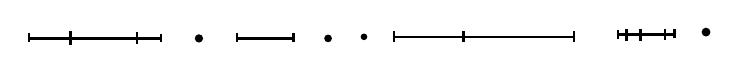
\begin{tikzpicture}[x=0.8cm,y=1cm,line width=0.85pt]
\draw (0,0)--(2.1,0);
\draw (0,-0.05)--(0,0.07) (0.66,-0.08)--(0.66,0.09) (1.72,-0.07)--(1.72,0.08) (2.1,-0.04)--(2.1,0.06);
\fill (2.7,0) circle (1.5pt);
\draw (3.3,0)--(4.2,0);
\draw (3.3,-0.05)--(3.3,0.07) (4.2,-0.05)--(4.2,0.07);
\fill (4.75,0) circle (1.4pt);
\fill (5.32,0.02) circle (1.2pt);
\draw (5.8,0.02)--(8.65,0.02);
\draw (5.8,-0.04)--(5.8,0.09) (6.9,-0.04)--(6.9,0.09) (8.65,-0.04)--(8.65,0.09);
\draw (9.35,0.05)--(10.25,0.05);
\draw (9.35,-0.01)--(9.35,0.11) (9.49,-0.03)--(9.49,0.12) (9.71,-0.03)--(9.71,0.12) (10.1,-0.02)--(10.1,0.12) (10.25,0)--(10.25,0.12);
\fill (10.75,0.08) circle (1.6pt);
\end{tikzpicture}}

Dans CF III, j'ai pris la peine \unsure{essentiellement|éventuellement} de définir le support d'un tel objet comme partie de $I$ (appelée \deleted{\unsure{tout}} ``modérée \unsure{fermée}'', alors que j'aurais dû dire ``modérée'' tout court, et appeler \uline{constructibles} les parties que j'y appelle ``modérées''). Cela donne lieu à un formalisme raisonnable dans le cas \unsure{present|présent|provenant} d'un ens \inserted{fini} de figures ayant la propriété spécifiée au début. Dans le cas d'un ensemble infini, c'est OK si $I$ est un \uline{tronçon} ordonné (loc. cit. p.8) et encore --- toujours est-il que l'on trouve une notion de \uline{parties constructibles} de $I$, de complémentaire d'une telle partie, \deleted{et pour} une notion de compatibilité de parties constructibles, et un bon formalisme des $\bigcup_i,\ \bigcap_i,\ \unsure{\complement|C}$ pour des parties \unsure{constr.|constr} \inserted{$X_\alpha$} deux à deux \deleted{disjointes} compatibles (i.e. telles que la réunion des $\partial X_\alpha$ soit tot.\textsuperscript{t} ordonnée).
